\documentclass[a4paper]{article}
\usepackage{amsmath}
\usepackage{graphicx}
\usepackage{longtable}
\usepackage{makecell}
\usepackage[most]{tcolorbox}
\usepackage{listings}
\usepackage{csquotes}

\title{DRLND Continuous Control- Report}
\date{2018-12-09}
\author{Matthias Schinacher matthias.schinacher@googlemail.com}

\begin{document}

\maketitle
\tableofcontents
\newpage

\section{Intro}
The project is a homework assignment for Udacity's \textbf{Deep Reinforcement Learning Nano Degree}.
The project ist the second one called \textit{Continuous Control}.
\\
The project environment is a course provided version of the Unity "Reacher"
environment of the ML- agents Unity has on the respective github- page.
The environment has an "agent" - a robotic arm - which can be manipulated
using 4 continuous-value actions with range -1.0 to 1.0 that must be provided
at each timestep.
\\
The environemt also contains a slowly moving ball- shaped target area,
that the robotic arm must hit with it's end (it's hand?).
The longer the robot keeps being in the target area with the hand,
the higher the reward.
\\
For this project I chose to implement DDPG with experience replay and
a variant of priority replay in a python script to be invoked from command line.
\\
I developed the script initially from the one I wrote for the Navigation- project,
as there was a lot of overlap in how the assignments were structured (like
a unity agent with a similar API that needs to maximize rewards over a
number of episodes).
\\
The DDPG needs 4 approximations (actor, critic and the 2 target- variants of them)
that I modeled as neural networks with fully connected layers, ReLU layers,
$Tanh$- layers and batch-norm ("BatchNorm1") layers using PyTorch.

\subsection{Amendment 2018-12-11 (version 2)}
My attempt to solve the 1 agent environment were not conclusivly successful
and the reviewer suggested to try the 20 agent version.
\\
So I did that, the updates to the report are market by
\textbf{Amendment 2018-12-11 (version 2)}.

\section{Implementation}
\subsection{Python script}
The script is named $ms\_drlndcc\_pr.py$ and must be invoked from the command
line with exactly one parameter, the name of the ".ini"- file (a.k.a. command file),
that has all the parameters.
\\
\textbf{Amendment 2018-12-11 (version 2):} I implemented an additional variant
of the script for the 20 agent version of the \enquote{Reacher} environment
called $ms\_drlndcc\_pr\_20.py$.

\paragraph{Parameters}
The parameters listed in the command file come in various sections. The basic format
is similar to the Windows style INI files and is the one that pythons $configparser$
module uses (as the module is used in the script).

\subparagraph{Example}
:\\
\tiny
\texttt{
{[global]} \\
runlog = test06.log \\
{[mode]} \\
train = True \\
{[rand]} \\
seed = 32177 \\
{[model]} \\
h1 = 237 \\
h2 = 237 \\
c\_h1 = 237 \\
c\_h2 = 237 \\
load\_file = test05 \\
save\_file = test06 \\
{[hyperparameters]} \\
episodes           = 50 \\
warmup\_episodes    = 5 \\
warmup\_episodes\_f  = 0.5 \\
replay\_batchsize   = 64 \\
replay\_steps       = 5 \\
optimizer\_steps    = 5 \\
tau                = 0.001 \\
reward\_gamma       = 0.95 \\
reward\_offset      = 0.01 \\
no\_reward\_rm\_prob  = 0.05 \\
epsilon\_start      = 0.3 \\
epsilon\_delta      = 0.000001 \\
epsilon\_min        = 0.0031
}

\normalsize

\subparagraph{Description}
:\\
\small
\begin{tabular}{ |l|r|l|c| }
  \hline
  \multicolumn{4}{|c|}{Parameters} \\
  \hline
Section & Name & Description & Default \\
  \hline
\multicolumn{4}{|l|}{\textbf{global}} \\
               & runlog & name of the logfile to use & \texttt{run.log} \\
\multicolumn{4}{|l|}{\textbf{mode}} \\
               & train & whether we're in training mode & \texttt{True} \\
               & show & \makecell[tl]{flag, whether to show \\ the simulation in "human time"} & \texttt{False} \\
\multicolumn{4}{|l|}{\textbf{rand}} \\
               & seed & \makecell[tl]{seed for \\ random number generation} & \makecell[tc]{no explicit \\ random seeding performed} \\
\multicolumn{4}{|l|}{\textbf{model}} \\
               & h1 & \makecell[tl]{first size- parameter \\ for the actor- NN- model} & \texttt{10} \\
               & h2 & \makecell[tl]{second size- parameter \\ for the actor-NN- model} & \texttt{10} \\
               & c\_h1 & \makecell[tl]{first size- parameter \\ for the critic- NN- model} & \texttt{10} \\
               & c\_h2 & \makecell[tl]{second size- parameter \\ for the critic-NN- model} & \texttt{10} \\
               & load\_file & \makecell[tl]{name- fragment for the files \\ from which to load models (if any)} & None \\
               & save\_file & \makecell[tl]{name- fragment for the files \\ to save the models to} & \makecell[tc]{"\texttt{DDPG-out}" \\ if in training mode} \\
\multicolumn{4}{|l|}{\textbf{hyperparameters}} \\
               & episodes & number of episodes to run & \texttt{200} \\
               & warmup\_episodes & \makecell[tl]{epiosodes to run with \\ pure random sampling} & \texttt{10} \\
               & warmup\_episodes\_f & \makecell[tl]{scale factor for pure random sampling} & \texttt{0.4} \\
               & replay\_buffersize & size of the replay memory & \texttt{99000} \\
               & replay\_batchsize & \makecell[tl]{number of transitions to sample \\ per optimizing step} & \texttt{128} \\
               & replay\_steps & \makecell[tl]{simulation-steps between \\ each optimization run} & \texttt{20} \\
               & optimizer\_steps & \makecell[tl]{no. of batch optimization-steps \\ per optimization run} & \texttt{10} \\
               & learning\_rate & the learning rate & \texttt{0.001} \\
               & gamma & $\gamma$ & \texttt{0.99} \\
               & tau & $\tau$ (soft target update) & \texttt{0.001} \\
\multicolumn{4}{|c|}{\textit{replay prioritization}} \\
               & reward\_gamma & reward- $\gamma$ discount factor & \texttt{0.99} \\
               & reward\_offset & importance offset & \texttt{0.01} \\
               & no\_reward\_rm\_prob & \makecell[tl]{probability for transition \\ with zero- reward \\ to enter replay- memory} & \texttt{0.25} \\
\multicolumn{4}{|c|}{\textit{sample action noise}} \\
               & epsilon\_start & start value for $\epsilon$ & \texttt{0.5} \\
               & epsilon\_delta & \makecell[tl]{value to subtract from $\epsilon$ \\ for each optimization step} & \texttt{0.5} \\
               & epsilon\_min & minimum/ final value for $\epsilon$ & \texttt{0.001} \\
               & noise\_theta & $\theta$ for noise process & \texttt{0.15} \\
               & noise\_sigma & $\sigma$ for noise process & \texttt{0.02} \\
%               &  &  & \texttt{} \\
\hline
\end{tabular}
\normalsize
\\
\textbf{Note:} the $show$- parameter determines, if the unity engine should
show the episodes slower, as to allow a human observer to follow the simulation; therefor
it determines the value given to the unity- environment as the parameter $train\_mode$.
\\
The $train$- parameter of the script determines, if the algorithm will be learning
from new transitions.

\subsection{Dependencies}
The script has runtime dependencies; these are the ones as described in the
project instructions; I will therefore refrain from detailing the dependencies \textit{here}.

\subsection{Details/ algorithm}
The algorithm implemented is basically Deep Deterministic Policy Gradient (DDPG)
with a few tweaks.
\\
The replay memory-buffer is implemented as a simple list with a specified capacity (\textit{replay\_buffersize}),
where the oldest entry is overwritten by the newest entry, if the capacity is already
fully used.
\\
The script uses a specified number (\textit{replay\_batchsize}) of transitions
to perform the optimization step; how often the optimization step is performed
is determined by \textit{replay\_steps}, that is once every \textit{replay\_steps}
simulation-steps the optiization is performed, and \textit{optimizer\_steps}
controls how many batches/ optimization steps are performed in sequence then.
\\
Also the script implements an unusual non standard form of priority replay
as well as a noise adjustment of the sampled actions.

\paragraph{Priority replay}
Different from the usual priority replay, where the sampling probability of the
transition is governed by "how unexpected" the transition was (difference between
actual reward and reward expected by the current state value function) I implemented
a prioritization based on the actual reward only. This scheme has 3 elements:
\begin{itemize}
\item a transition with zero reward is only registered to replay memory
with a certain probability (\textit{no\_reward\_rm\_prob});
transitions with reward greater zero are always registered.
\item sampling probability from the replay buffer for a batch is relative
to the transition-reward plus a reward offset (\textit{reward\_offset}, to allow
for sampling of zero reward transitions)
\item the rewards used to compute the sampling probability are discounted by
the reward- $\gamma$ factor in each optimization run to favor newer transitions.
\end{itemize}

\paragraph{Warmup episodes}
The script/ program computes the action values to be used randomly for
a number episodes (\textit{warmup\_episodes}), before the actual actor- model
is used. The values are sampled from the standard normal distribution and
mupltiplied by the factor \textit{warmup\_episodes\_f} before they are clipped
to the range -1 to 1.

\paragraph{Sampling noise}
When not in warmup, the action values are computed using the actor model,
to which a noise (times $\epsilon$) is added. The noise is computed by
$noise = noise -\theta noise + \sigma random\_number$. This noise is
initialized with zero and the \textit{random\_number} is taken from the
usual uniform distribution between 0 and 1.
\\
As the $\epsilon$ factor decreases the actual noise applied decreases also.

\paragraph{Neural Network layout}
The approximation functions for the actor and critic (the \textit{normal}
and the target variants) are implemented as neural networks using PyTorch.
\\
Each uses 3 linear layers with ReLU- layers after the first and second linear
layers and a batch-norm layer before the first linear layer.
The actor model has a final $tanh()$- layer (the critic does not).
The critic inputs the only the state to the first layers and mixes the action-
input after the first ReLU by concatinating it to the ReLU layers output
(before it goes intu the second linear layer).
\\

\begin{tabular}{ |c|c| }
  \hline
  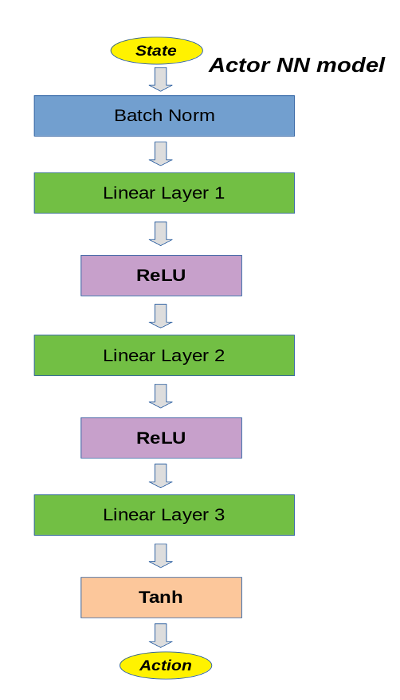
\includegraphics[scale=0.3]{ActorPic.png} & 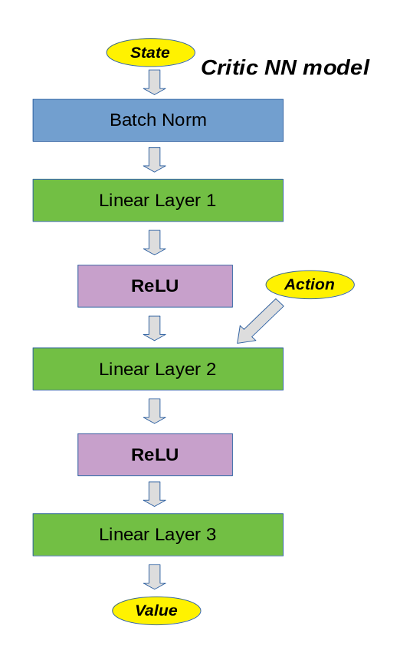
\includegraphics[scale=0.3]{CriticPic.png} \\
  \hline
\end{tabular}

\textbf{Note:} with 3 linear layers each and fixed sizes for the input
(by the unchangable values for state size and action size) as well as output
(action size and 1, cause the critic must yield a value), there are 2
choosable sizes for the actor and critic each (hence the parameters).

\subsection{Usage}
The script is invoked from the command line as a python script with one parameter,
a file-name from which to read all the parameters governing the algorithm.
\\
Example:\\
\texttt{python ms\_drlndcc\_pr.py test05.ini}
\\
\textbf{Amendment 2018-12-11 (version 2):} for the 20 agent version ...\\
\texttt{python ms\_drlndcc\_pr\_20.py test05\_20.ini}

\subsection{Loading and saving models/ pretraining}
The script is able to save the model- states of the neural networks as well as
the transitions in the replay-memory to file and/or load these from file
at the beginning of a script-run.
\\
The parameters allow for a name- fragment to be specified, from which the
actual filenames are derived. Each NN- model as well as the transitions-
replay buffer (plus reward- buffer) gets it's seperate file.
\\
The models are saved/ loaded using PyTorch's build in mechanism and the
replay- buffer file is created using pythons \textit{pickle}- module.

\small
\begin{tabular}{ |l|l| }
  \hline
  \multicolumn{2}{|c|}{file names} \\
  \hline
data & physical file name \\
  \hline
actor model & \texttt{actor\_\{fragment\}.model} \\
target actor model & \texttt{target\_actor\_\{fragment\}.model} \\
critic model & \texttt{critic\_\{fragment\}.model} \\
target critic model & \texttt{target\_critic\_\{fragment\}.model} \\
replay buffer & \texttt{transitions\_\{fragment\}.pickle} \\
  \hline
\end{tabular}
\normalsize

The saved model/ transitions allow for a subsequent script/ program- run to
pick up, where a previous run ended, effectivly using this as a pretraining.
This also allows to continue a simulation-run with adjusted algorithm parameters;
the neural net size parameters are ignored when loading aprevous model!

\subsection{Outputs}

The script prints some info to the standard output, but the actually important
output is the run-log file; it prints a (non '\#'-) textline per episode containing
the episode, the score the episode reached, the average score of the last 100
episodes (or 0, if it's an episode before the 100th), the minimum of all
non zero rewards for a single step, the maximum reward for a single step
the replay buffer size at the end of the episode and $\epsilon$ for the episode
separated by a blank.
The logfile can thus be read by certain programs/ tools as some sort
of time-series for the score and the average-100-last-episodes-score; one such
tool is \textbf{gnuplot}, with which I created the graphics contained in the report.

\subsection{Misc. algorithm details}
The algorithm distinguishes between \textbf{optimization run} and \textbf{optimization step}.
A optimization run occurs every \textit{replay\_steps} (when not in warmup) and
contains \textit{optimization\_steps} steps. Each such step uses a freshly sampled
batch from the replay buffer to feed it to the models as the DDPG algorithm
prescribes; 2 instances of the PyTorch Adam- optimizer are used to make a step
for actor and critic.
\\
\textbf{Note:} the target networks are soft- updated per optimization step,
and the $\epsilon$ for the action noise is also adjusted per step, while
the rewards for the prioritization of the replay buffer are discounted per
optimization run.

\section{Results}
\subsection{Target score}
To my big disappointment, the target score of 30 never even remotly materialized
with my experiments/ simulations. I don't think a faster computer with maybe
a real GPU (I used my laptop to run the simulations) would have gotten me there
even though it would allow for longer runs and bigger or deeper networks.
\\
But I do think, that the Reacher- environment I used \textbf{does not yield
rewards of 0.1 per timestep, when the robot arm is in the target area!}
I think, that it must either be a different environment compared to the one
used to establish the score of 30, or there is some subtle dependency on
the operating system I use (a variant of Ubuntu 18.04) or other software
installed locally, that alters these rewards, that are returned.
\\
I must stress, that I downloaded the environment more than twice from the
location given in the instructions; this can not be the source of this problem
(I mean a different Reacher environment).
\\
I very purposely let my script print out the maximum and minimum reward
(other than zero) returned by the environment per step for each episode,
and the typical values are $0.039999999...$ and $0.009999999...$, but never $0.1$.
\\
\textbf{Amendment 2018-12-11 (version 2):} as suggested by the reviewer, I
tried the 20 agents environment instead of the 1 agent environment.
TODO: describe in more detail (simulation still running)

\subsection{General remarks}
I had some problems to get to the point where my implementation would yield
a simulation-run, that actually clearly demonstrated learning. My DDPG implementation
seems to behave quite fickle and is very sensitive regarding the \textit{right}
choice of parameters.\\
It seems to me that others had similar problems, therefor I guess this is
mainly due to the DDPG algorithm as such in combination with the Reacher environment :-).
\\
I was then very happy to have found some parameter combinations, where my
script would show learning. I did try a variety of different things before
I got to this point, not all of which are reflected in the final version
of the python script since I deleted them after they did not yield
the results I had hoped (plus one or two of these ideas were clearly bonkers
to start with, I realize in hindsight).

\subsection{Results of selected simulation runs}

\textbf{Amendment 2018-12-11 (version 2):} I added the results for the two
simulations with the 20 agents variant.

\paragraph{Command files/ INI- files}
Each command file (a.k.a. INI- file) represents one \textit{experiment} (program/ script- run).
See the list below for an overview of these experiments/ command files
(refer to the actual files for details of all hyperparameters).
\\

\begin{tabular}{ |l|l| }
  \hline
Filename & Description \\
  \hline
$test07.ini$ & \makecell[tl]{first successful simulation with actual learning \\ with size- parameters $h1$ and $h2$ each 117 \\ (actor and critic)} \\
$test08.ini$ & \makecell[tl]{continuation of $test07.ini$, uses model \\ from latter as pre-training \\ different hyper-parameters \\ shows almost no learning!} \\
$test09.ini$ & \makecell[tl]{second successful simulation \\ actor and critic with different \\ linear layer sizes } \\
$test09b.ini$ & \makecell[tl]{continuation of $test09.ini$, uses model \\ from latter as pre-training \\ different hyper-parameters} \\
$test09c.ini$ & \makecell[tl]{continuation of $test09.ini$, uses model \\ from latter as pre-training \\ different hyper-parameters} \\
$test09d.ini$ & \makecell[tl]{continuation of $test09.ini$, uses model \\ from latter as pre-training \\ different hyper-parameters} \\
  \hline
$test10_20.ini$ & \makecell[tl]{with parameters suggested by the reviewer \\ for the 20 agents variant} \\
$test10_20b.ini$ & \makecell[tl]{with some other parameters \\ for the 20 agents variant} \\
  \hline
\end{tabular}

\paragraph{Graph- plots}

\textit{(All plots are score per episode plus average score of the last 100 episodes per episode.
All plots for the same variant - 1 or 20 agents -are ploted with the same x/y- max/min- values
for comparability. Constants of 4 and 30 are plotted as reference points.)}
\\
\begin{tabular}{ |c|c| }
  \hline
  \texttt{test07.ini} & \texttt{test08.ini} \\
  \hline
  \includegraphics[scale=0.35]{test07.png} & \includegraphics[scale=0.35]{test08.png} \\
  \hline
\end{tabular}
\\
\begin{tabular}{ |c|c| }
  \hline
  \texttt{test09.ini} & \texttt{test09b.ini} \\
  \hline
  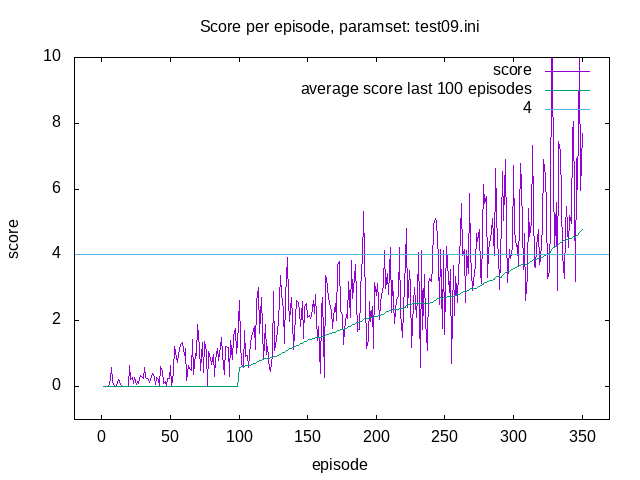
\includegraphics[scale=0.35]{test09.png} & \includegraphics[scale=0.35]{test09b.png} \\
  \hline
  \texttt{test09c.ini} & \texttt{test09d.ini} \\
  \hline
  \includegraphics[scale=0.35]{test09c.png} & \includegraphics[scale=0.35]{test09d.png} \\
  \hline
\end{tabular}
\\
\begin{tabular}{ |c|c| }
  \hline
  \texttt{test10\_20.ini} & \texttt{test10\_20b.ini} \\
  \hline
  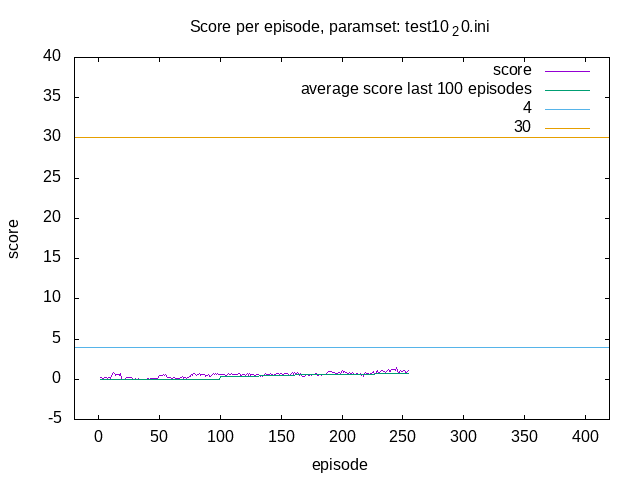
\includegraphics[scale=0.35]{test10_20.png} & \includegraphics[scale=0.35]{test10_20b.png} \\
  \hline
\end{tabular}

\subsection{Remarks/ discussion}
The \texttt{test07.ini} simulation shows clear learning and reaches a sustained
score of about 4 before mildly \enquote{crashing} at about episode 250. I'm frankly
not able to say why it goes down like this.
\\
Though \texttt{test08.ini} uses the identical model sizes and only sligthly
different other hyperparameters, it is not able to learn nearly in the same
way. I suspect the main difference to be the changed minimum $\epsilon$ noise
parameter. Anyhow, I think it shows the sensivity of the algorithm towards
changes in these parameters.
\\
\texttt{test09.ini} on the other hand seems to learn more slowly than
\texttt{test07.ini}, but also more \enquote{sustainable} (does not go down).
The main difference being a much larger batch size and different sizes for
the NN- layers, where the 2 size parameters is different (first layer decidedly
bigger than the second one) for the actor and critic models; also the
size parameters differ between actor and critic.
\\
At first look, one would think, the \texttt{test09.ini} run would yield even
higher scores, if it had been longer, since the average score is still climbing
at the end, but since \texttt{test09b.ini}, \texttt{test09c.ini} and
\texttt{test09d.ini} are continuations of it (same NN model structure), and they
seem to linger on the level reached or even sligthly go down, the score
reached seems to be about the best value I can get with my algorithm;
Thus about a sustained $5.3$- score is what I get.
\\
\textbf{Amendment 2018-12-11 (version 2):} TODO: discuss results
of the simulations for the 20 agents variant.

\subsection{Result models and data}
The neural network models for the simulations can be found in the respective
\texttt{*.model}- files, where they are saved in the PyTorch specific manner;
note that you need to use the \texttt{MSA} (actor) and \texttt{MSC} (critic)
classes within the script in addition to PyTorch.
\\
You can also kind of \enquote{print out} the models with the script
\texttt{print\_model.py}, but this will not give you all parameter values
out of the box (modify the script accordingly, if you want :-)).
\\
\subsection{ZIP files}
I zipped the resulting log-files, model files, transitions (replay buffer)- files
and INI- files in various \texttt{*.zip} archives.

\section{Possible improvements}
\subsection{Algorithm}
\paragraph{Random sampling/ noise}
The implementation uses a random-noise source to tweak the actions, that the
actor model computes for a state. I could think of 2 straightforward things one might try here:
\begin{itemize}
\item applying noise to the state (input) instead of the computed actions (output)
\item currently all 4 action dimensions are supplied with noise at each step;
this could be altered by randomly choosing not to apply noise per step or
applying noise not to all 4 actions; a variety of schemes are possible here.
\end{itemize}

\subparagraph{Tweaking $\epsilon$- decay}
Additionally, the $\epsilon$- decay for the noise was rather simple, a start value,
a minimum value and a delta to subtract per optimization step,
resulting in a linear decrease.
\\
The actual simulation results suggest, that the $\epsilon$- parameter
does have a serious impact on the algorithms performance;
thus other forms of $\epsilon$ decay (e.g. non linear) could be explored.

\paragraph{Priority replay}
The priority replay used seems a bit unusal. The idea was, that a step, where
we do get a reward is more important to further examine than one with zero
reward.
\\
Of course it would be interesting to see, whether a more traditional approach
to priority replay would yield different results.

\paragraph{Non DDPG}
Of course, because DDPG did not yield the results I wanted, maybe I should
try something else, maybe Q-Prop.

\subsection{NN- Models}
The models for the neural networks have considerable influence on the
performance of the simulation as a matter of course.
\\
My gut feeling is, that a much deeper network or bigger layers
would not be that promising, but maybe using a different activation function
for the actor (instead of $Tanh()$) or adding convolutional layers might smooth
the erratic score yield? This seems to me actually pretty similar to the
way my \textbf{Navigation}- project output behaved; coincidence?

\end{document}
